 %██████╗██╗   ██╗██████╗ ██╗   ██╗███████╗    ███████╗██╗████████╗████████╗██╗███╗   ██╗ ██████╗ 
%██╔════╝██║   ██║██╔══██╗██║   ██║██╔════╝    ██╔════╝██║╚══██╔══╝╚══██╔══╝██║████╗  ██║██╔════╝ 
%██║     ██║   ██║██████╔╝██║   ██║█████╗      █████╗  ██║   ██║      ██║   ██║██╔██╗ ██║██║  ███╗
%██║     ██║   ██║██╔══██╗╚██╗ ██╔╝██╔══╝      ██╔══╝  ██║   ██║      ██║   ██║██║╚██╗██║██║   ██║
%╚██████╗╚██████╔╝██║  ██║ ╚████╔╝ ███████╗    ██║     ██║   ██║      ██║   ██║██║ ╚████║╚██████╔╝
 %╚═════╝ ╚═════╝ ╚═╝  ╚═╝  ╚═══╝  ╚══════╝    ╚═╝     ╚═╝   ╚═╝      ╚═╝   ╚═╝╚═╝  ╚═══╝ ╚═════╝ 
%.:..:..:..:..:..:..:..:..:..:..:..:..:..:..:..:..:..:..:..:.
\section{Curve Fitting}



The equation for AWGN Curve fitting is:
\begin{align*}
	\begin{split}
y=f(x) = 0.0005046x^9 &+ 0.02122x^8 -0.02507x^7 - 0.1269x^6 + 0.1545x^5\\ &+ 0.2027x^4 - 0.3122x^3 + 0.049 x^2 - 0.004642
\end{split}
\end{align*}
\begin{mathDef}
	\mathSymb{x}{SNR value in dB.}
	\mathSymb{y}{BER}
\end{mathDef}
 
\begin{figure}[htpb!]
	\centerline{\resizebox{!}{0.5\textheight}{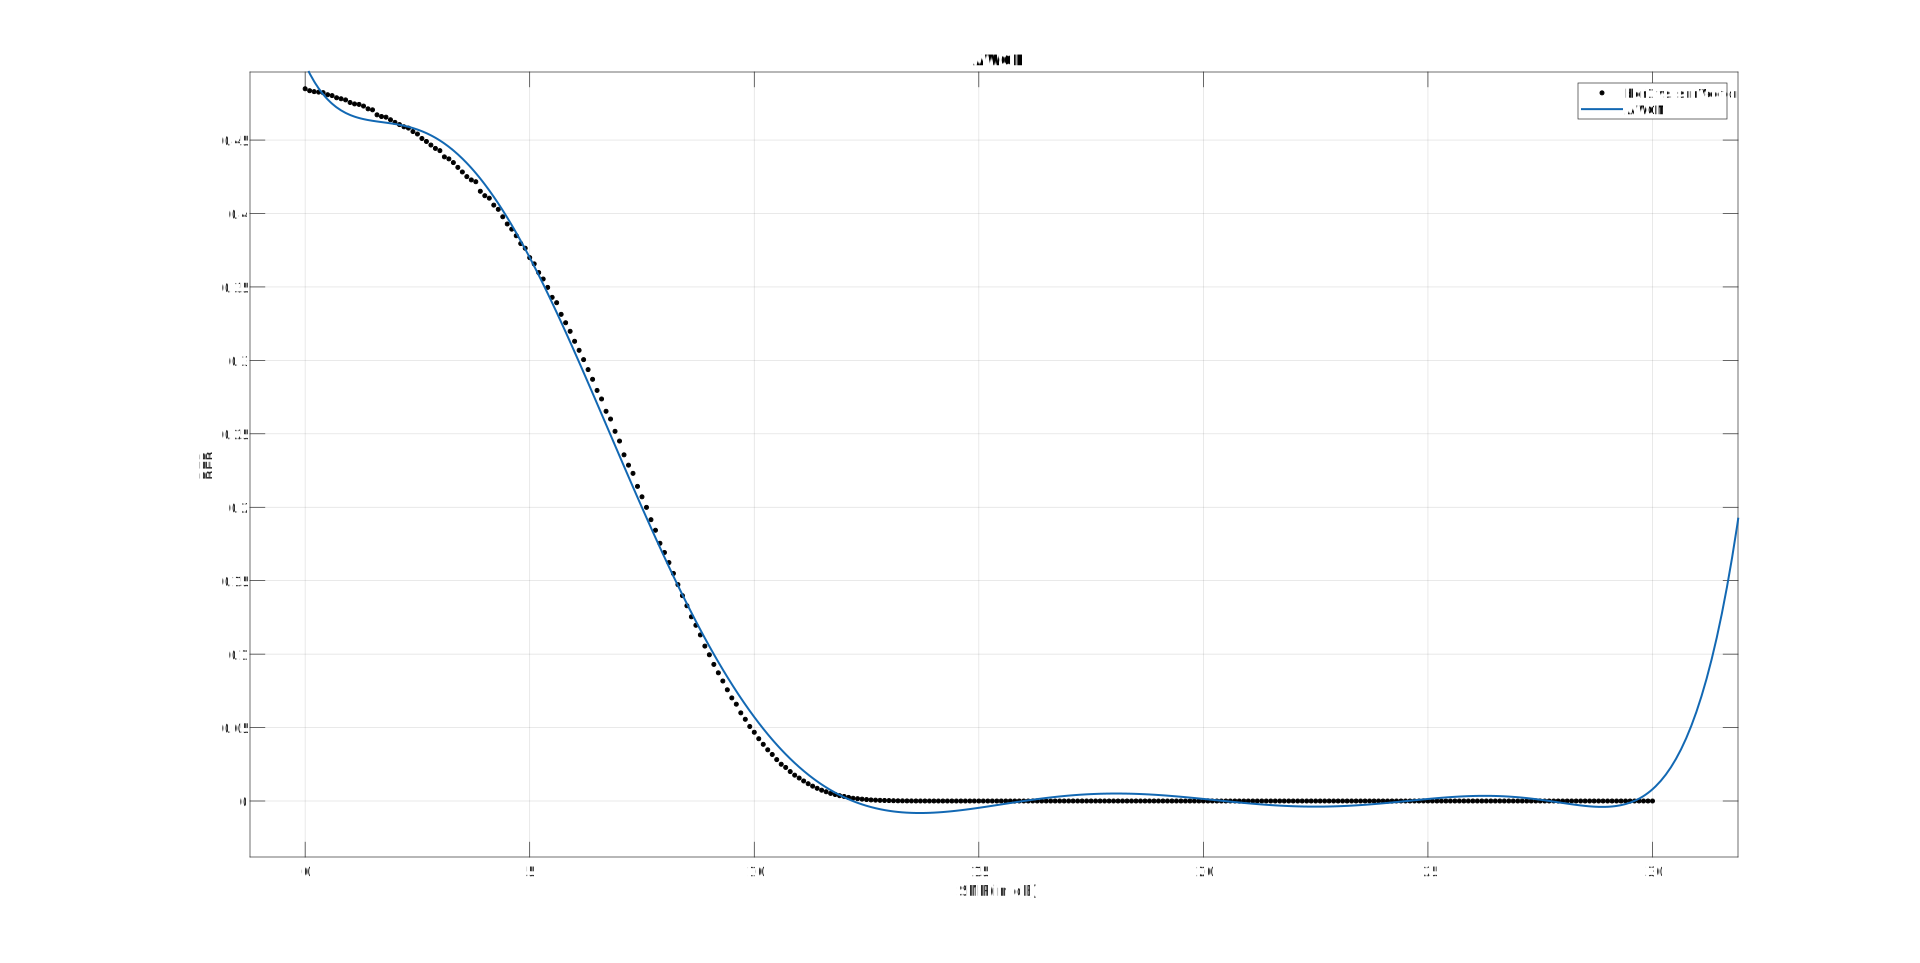
\includegraphics{Graphics/Results/AWGN.pdf}}}
	\caption{AWGN Curve Fitting}
	\label{fig:awgn_fit}
\end{figure}

\pagebreak


The equation for Rayleigh Curve fitting is:
\begin{align*}
\begin{split}
y=f(x) = 0.01108x^9 &- 0.01629x^8 - 0.07991x^7 + 0.123x^6 + 0.1912x^5\\& - 0.3401x^4 - 0.1262x^3 + 0.4212x^2 - 0.2217x + 0.03777
\end{split}
\end{align*}

\begin{figure}[htpb!]
	\centerline{\resizebox{!}{0.45\textheight}{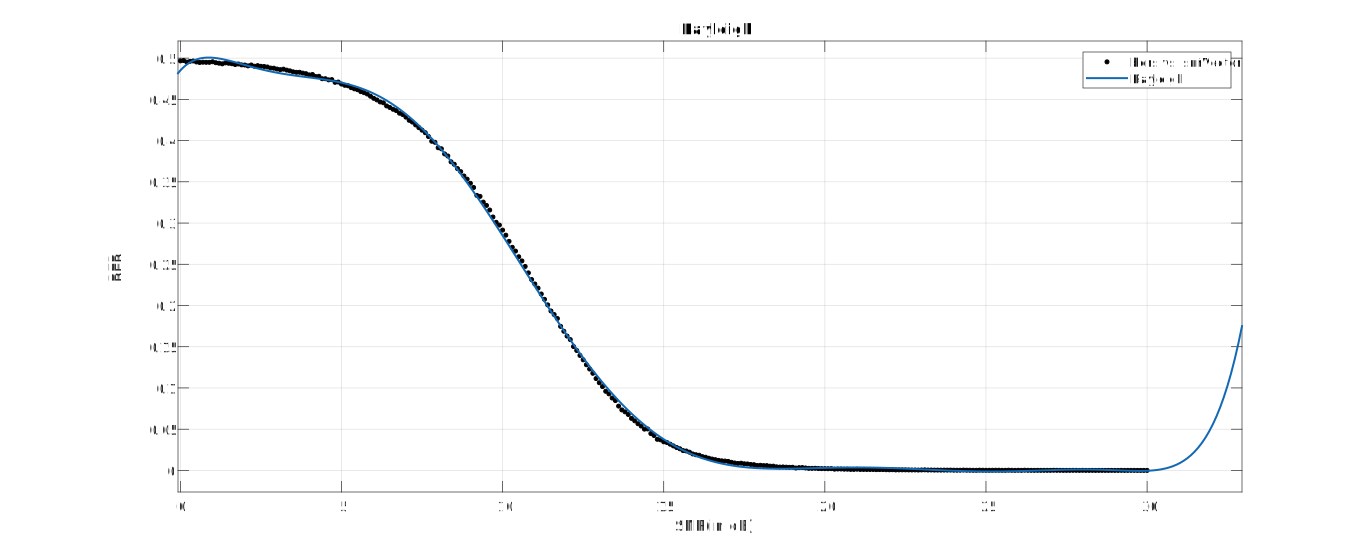
\includegraphics{Graphics/Results/Rayleigh.pdf}}}
	\caption{Rayleigh Curve Fitting}
	\label{fig:rayleigh_fit}
\end{figure}

\pagebreak

The equation for Rician Curve fitting is:
\begin{align*}
\begin{split}
	y=f(x) = 0.00643x^9 &+ 0.01816x^8 - 0.06692x^7 - 0.1026x^6 + 0.2525x^5\\& + 0.1372x^4 - 0.3881x^3 + 0.1103x^2 + 0.03639x - 0.006899
\end{split}
\end{align*}

\begin{figure}[htpb!]
	\centerline{\resizebox{!}{0.45\textheight}{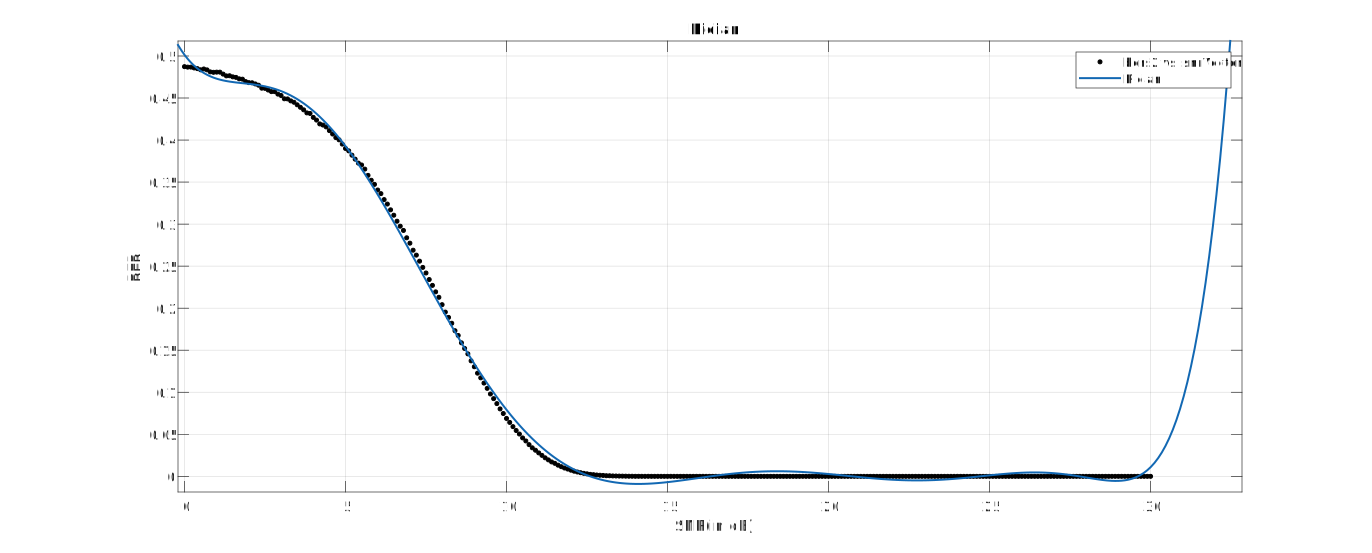
\includegraphics{Graphics/Results/Rician.pdf}}}
	\caption{Rician Curve Fitting}
	\label{fig:rician_fit}
\end{figure}

\pagebreak


